\chapter[Multicollinearity]{Multicollinearity in Species Distribution Modeling}

\begin{objetivos}
By the end of this chapter, readers should be able to explain multicollinearity
in SDM; identify redundant environmental variables using correlation; calculate
and interpret the variance inflation factor (VIF); understand the effects of
collinearity on ecological interpretation, parameter stability, and model
transferability; use principal component analysis (PCA) for dimensionality
reduction; and build a reproducible R workflow for selecting or transforming
environmental predictors before model fitting.
\end{objetivos}

\section{Introduction}

Multicollinearity occurs when two or more predictors carry similar information.
It is common in species distribution modeling because climatic, topographic,
edaphic, and hydrological variables frequently covary across space. Mean annual
temperature may be strongly associated with elevation, annual precipitation
with precipitation of the wettest quarter, and several topographic metrics may
be redundant because they derive from the same digital elevation model.

Strongly correlated predictors can produce unstable models, obscure variable
importance, inflate uncertainty in parametric models, and reduce spatial or
temporal transferability. Environmental-predictor selection should therefore
combine ecological reasoning, exploratory analysis, and statistical criteria
\parencite{guisan2017habitat,naimi2016sdm,raes2018modeling}.

\begin{atencao}[title={\faExclamationTriangle\quad More predictors do not necessarily produce a better model}]
Adding many environmental variables does not guarantee improved performance.
Redundant predictors may increase complexity, generate instability, hinder
ecological interpretation, and reduce transferability.
\end{atencao}

\section{The Multicollinearity Problem}

Environmental predictors often show strong mutual correlation. In tropical
regions, for example, high annual precipitation may coincide with low water
seasonality, while thermal gradients may follow elevation.

When two or more predictors carry similar information, multicollinearity
arises. Predictive performance may remain high, but ecological interpretation
of coefficients becomes unstable and spatial or temporal transfer may be
compromised \parencite{dormann2013collinearity}.

\section{Correlation Among Environmental Variables}

The simplest redundancy diagnostic is pairwise correlation. Pearson and
Spearman coefficients are the most common in SDM. Pearson measures linear
association between continuous variables. Spearman measures rank-based
monotonic association and is useful for nonnormal or skewed distributions.

Operational thresholds such as \(|r| > 0.7\) or \(|r| > 0.8\) are often used to
flag strong correlation. They are not universal rules. When two variables are
strongly correlated, preference should be given to the one with greater
ecological relevance, higher spatial quality, clearer interpretation, or better
alignment with the study objective
\parencite{dormann2013collinearity,raes2018modeling}.

\begin{conceito}[title={\faBook\quad Correlation is not causation}]
Two variables can be strongly correlated without either causing the other. In
SDM, correlation indicates shared information, but ecological knowledge and the
study hypothesis should determine which variable is retained.
\end{conceito}

\begin{conceito}[title={\faBook\quad Statistical correlation does not imply ecological redundancy}]
Strongly correlated variables may still represent distinct ecological
processes. Annual precipitation and precipitation of the driest quarter, for
example, may be correlated while representing different mechanisms related to
water availability.
\end{conceito}

\rscriptfile{scripts/unidade04/01_estrutura_pastas.R}
\rscriptfile{scripts/unidade04/02_preparar_variaveis_colineares.R}
\rscriptfile{scripts/unidade04/03_correlacao_variaveis.R}

\begin{figure}[H]
  \centering
  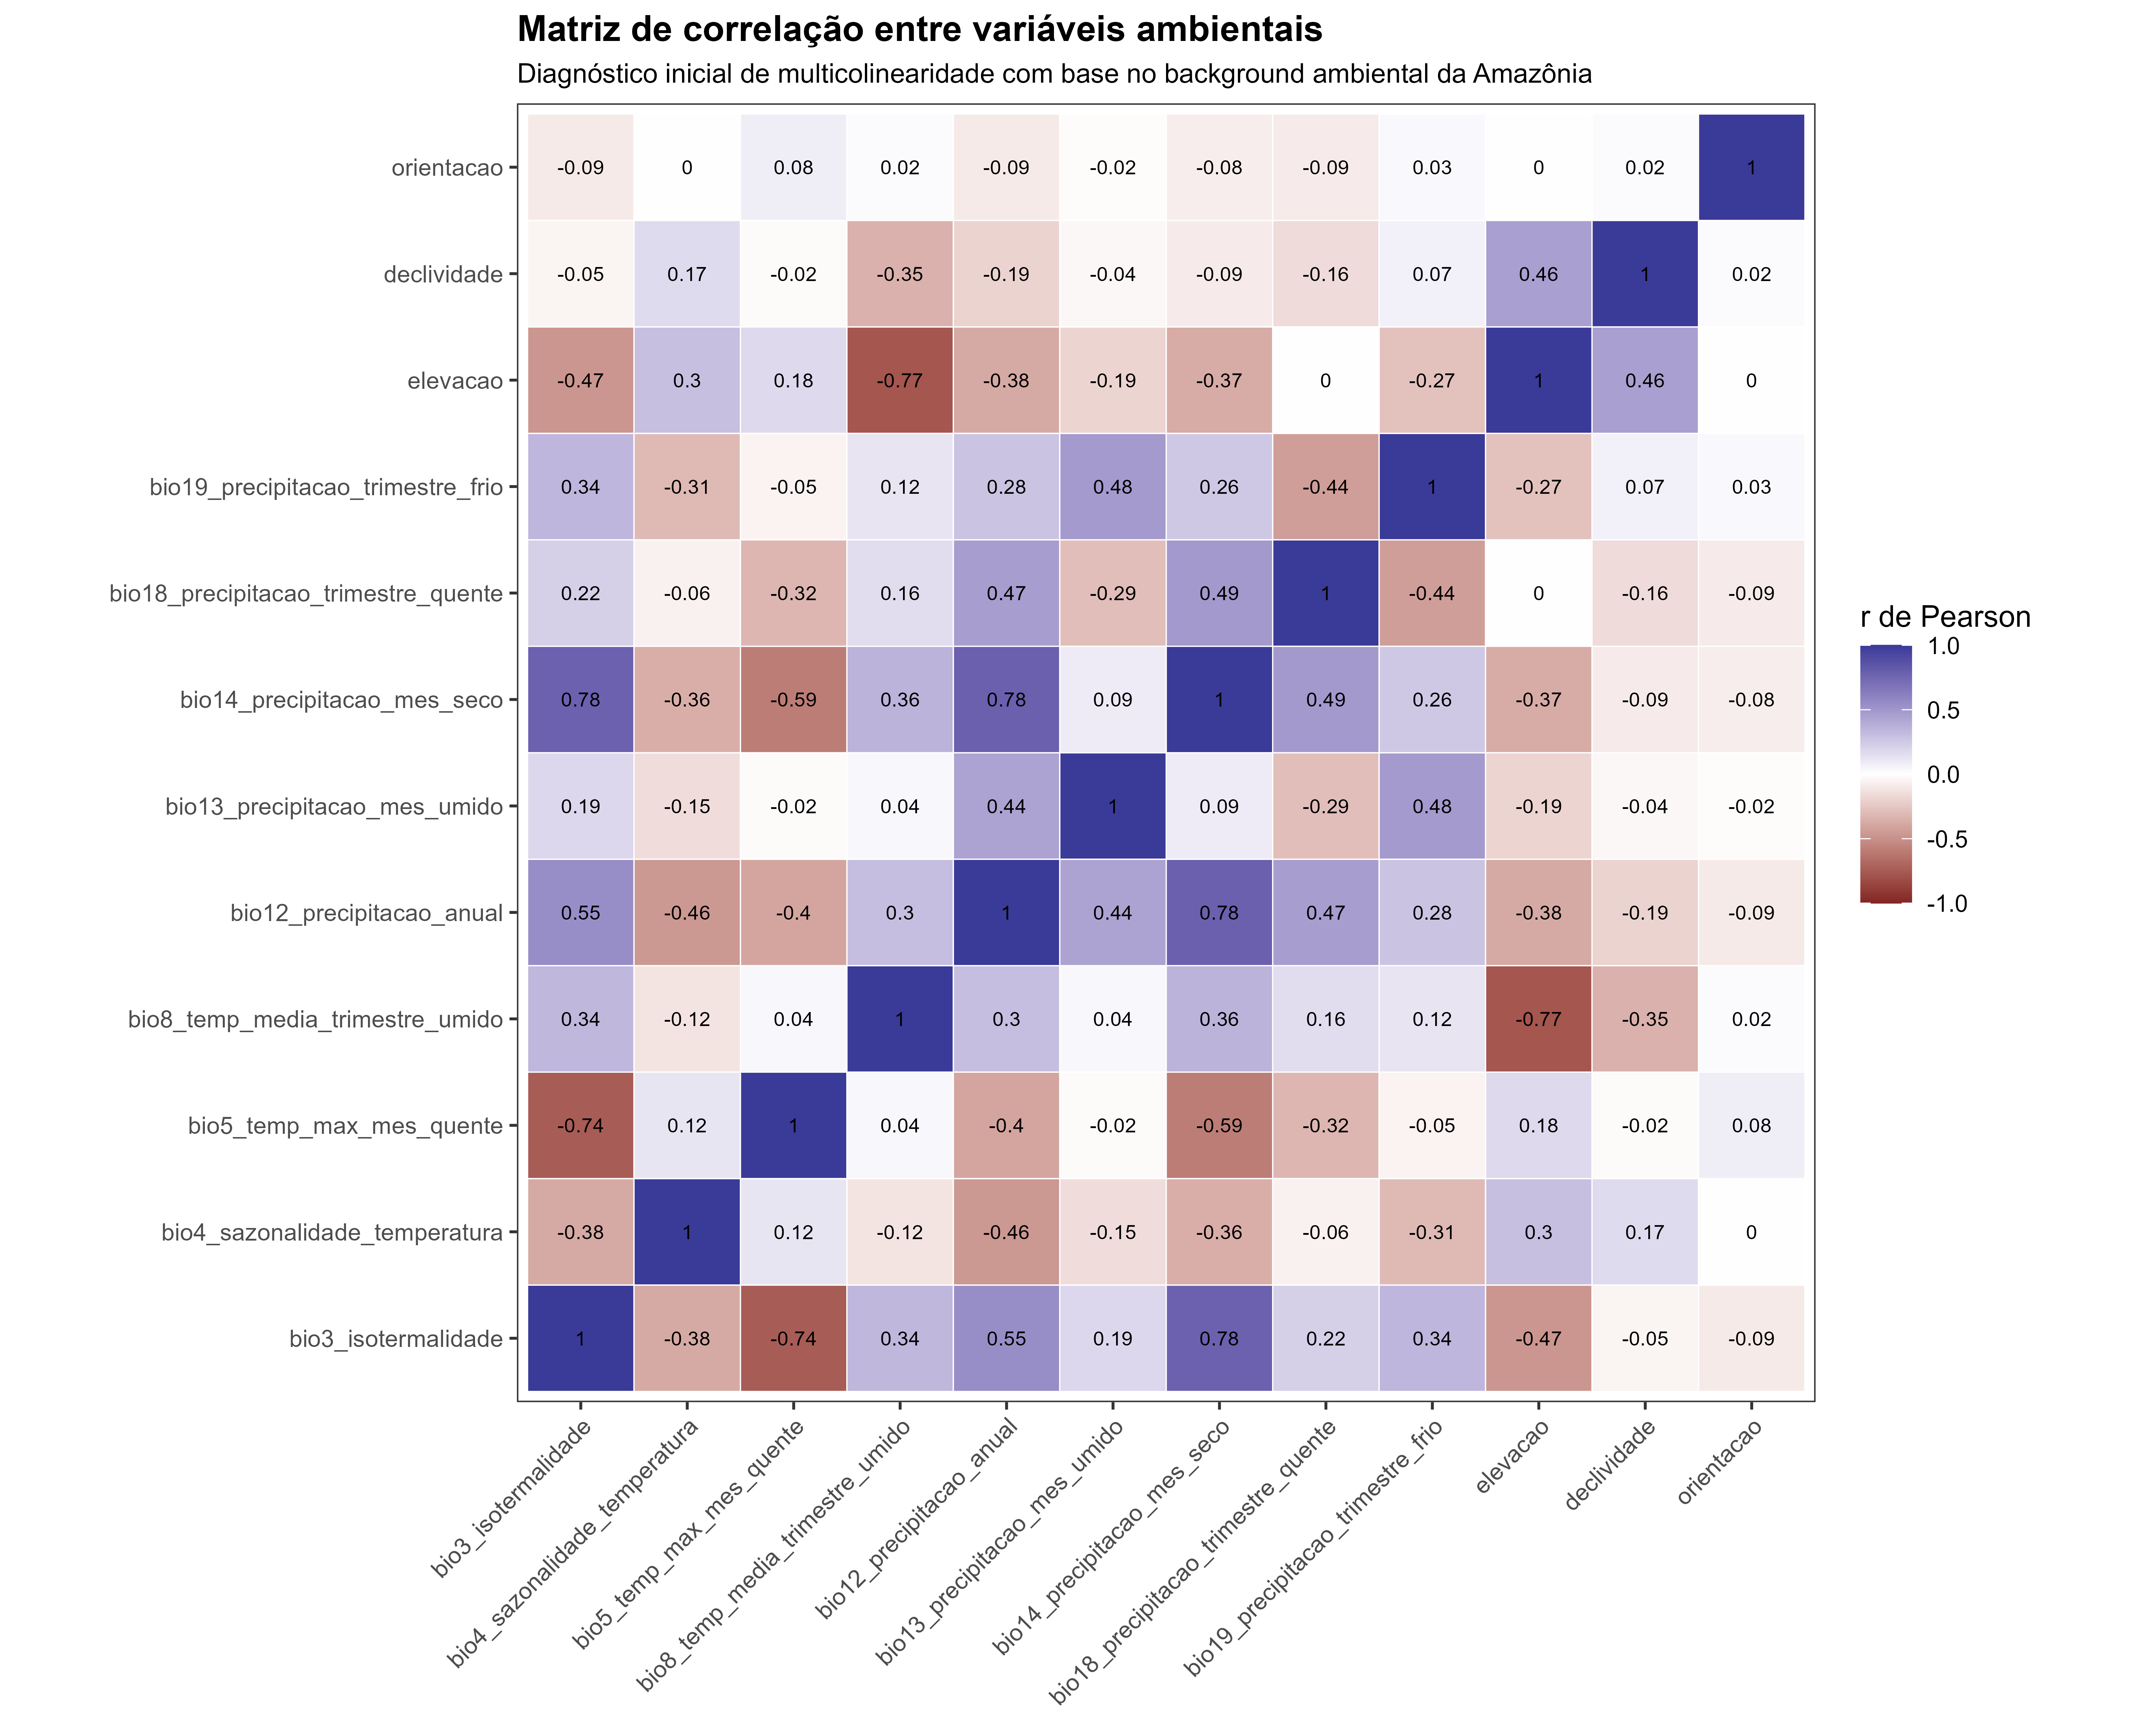
\includegraphics[width=\textwidth]{figuras/unidade04/unidade04_matriz_correlacao.png}
  \caption{Pearson correlation matrix for the environmental variables used to model \textit{Dinizia excelsa} across the Amazon biome. Coefficients indicate the strength of linear association between pairs of predictors.}
  \label{fig:unidade04_matriz_correlacao}
\end{figure}

\section{Variance Inflation Factor}

The variance inflation factor assesses how much the estimated variance of a
coefficient is inflated by linear dependence between one predictor and all
others. Unlike pairwise correlation, VIF evaluates each variable in relation to
the complete predictor set.

\begin{equationbox}
\[
VIF_j = \frac{1}{1 - R_j^2}
\]
Here, \(VIF_j\) is the variance inflation factor for predictor \(j\), and
\(R_j^2\) is the coefficient of determination from regressing predictor \(j\)
on all remaining predictors.
\end{equationbox}

High VIF indicates that a variable can be explained by a combination of the
others. A VIF above 10 is frequently interpreted as severe collinearity,
although more conservative thresholds such as 5 are also used in ecological
studies \parencite{obrien2007vif,dormann2013collinearity,naimi2016sdm}.

\begin{dica}[title={\faLightbulb\quad Correlation and VIF are complementary}]
Correlation identifies redundant pairs; VIF identifies redundancy relative to
the complete predictor set. Robust studies should examine both diagnostics.
\end{dica}

\rscriptfile{scripts/unidade04/04_vif_variaveis.R}

\begin{figure}[H]
  \centering
  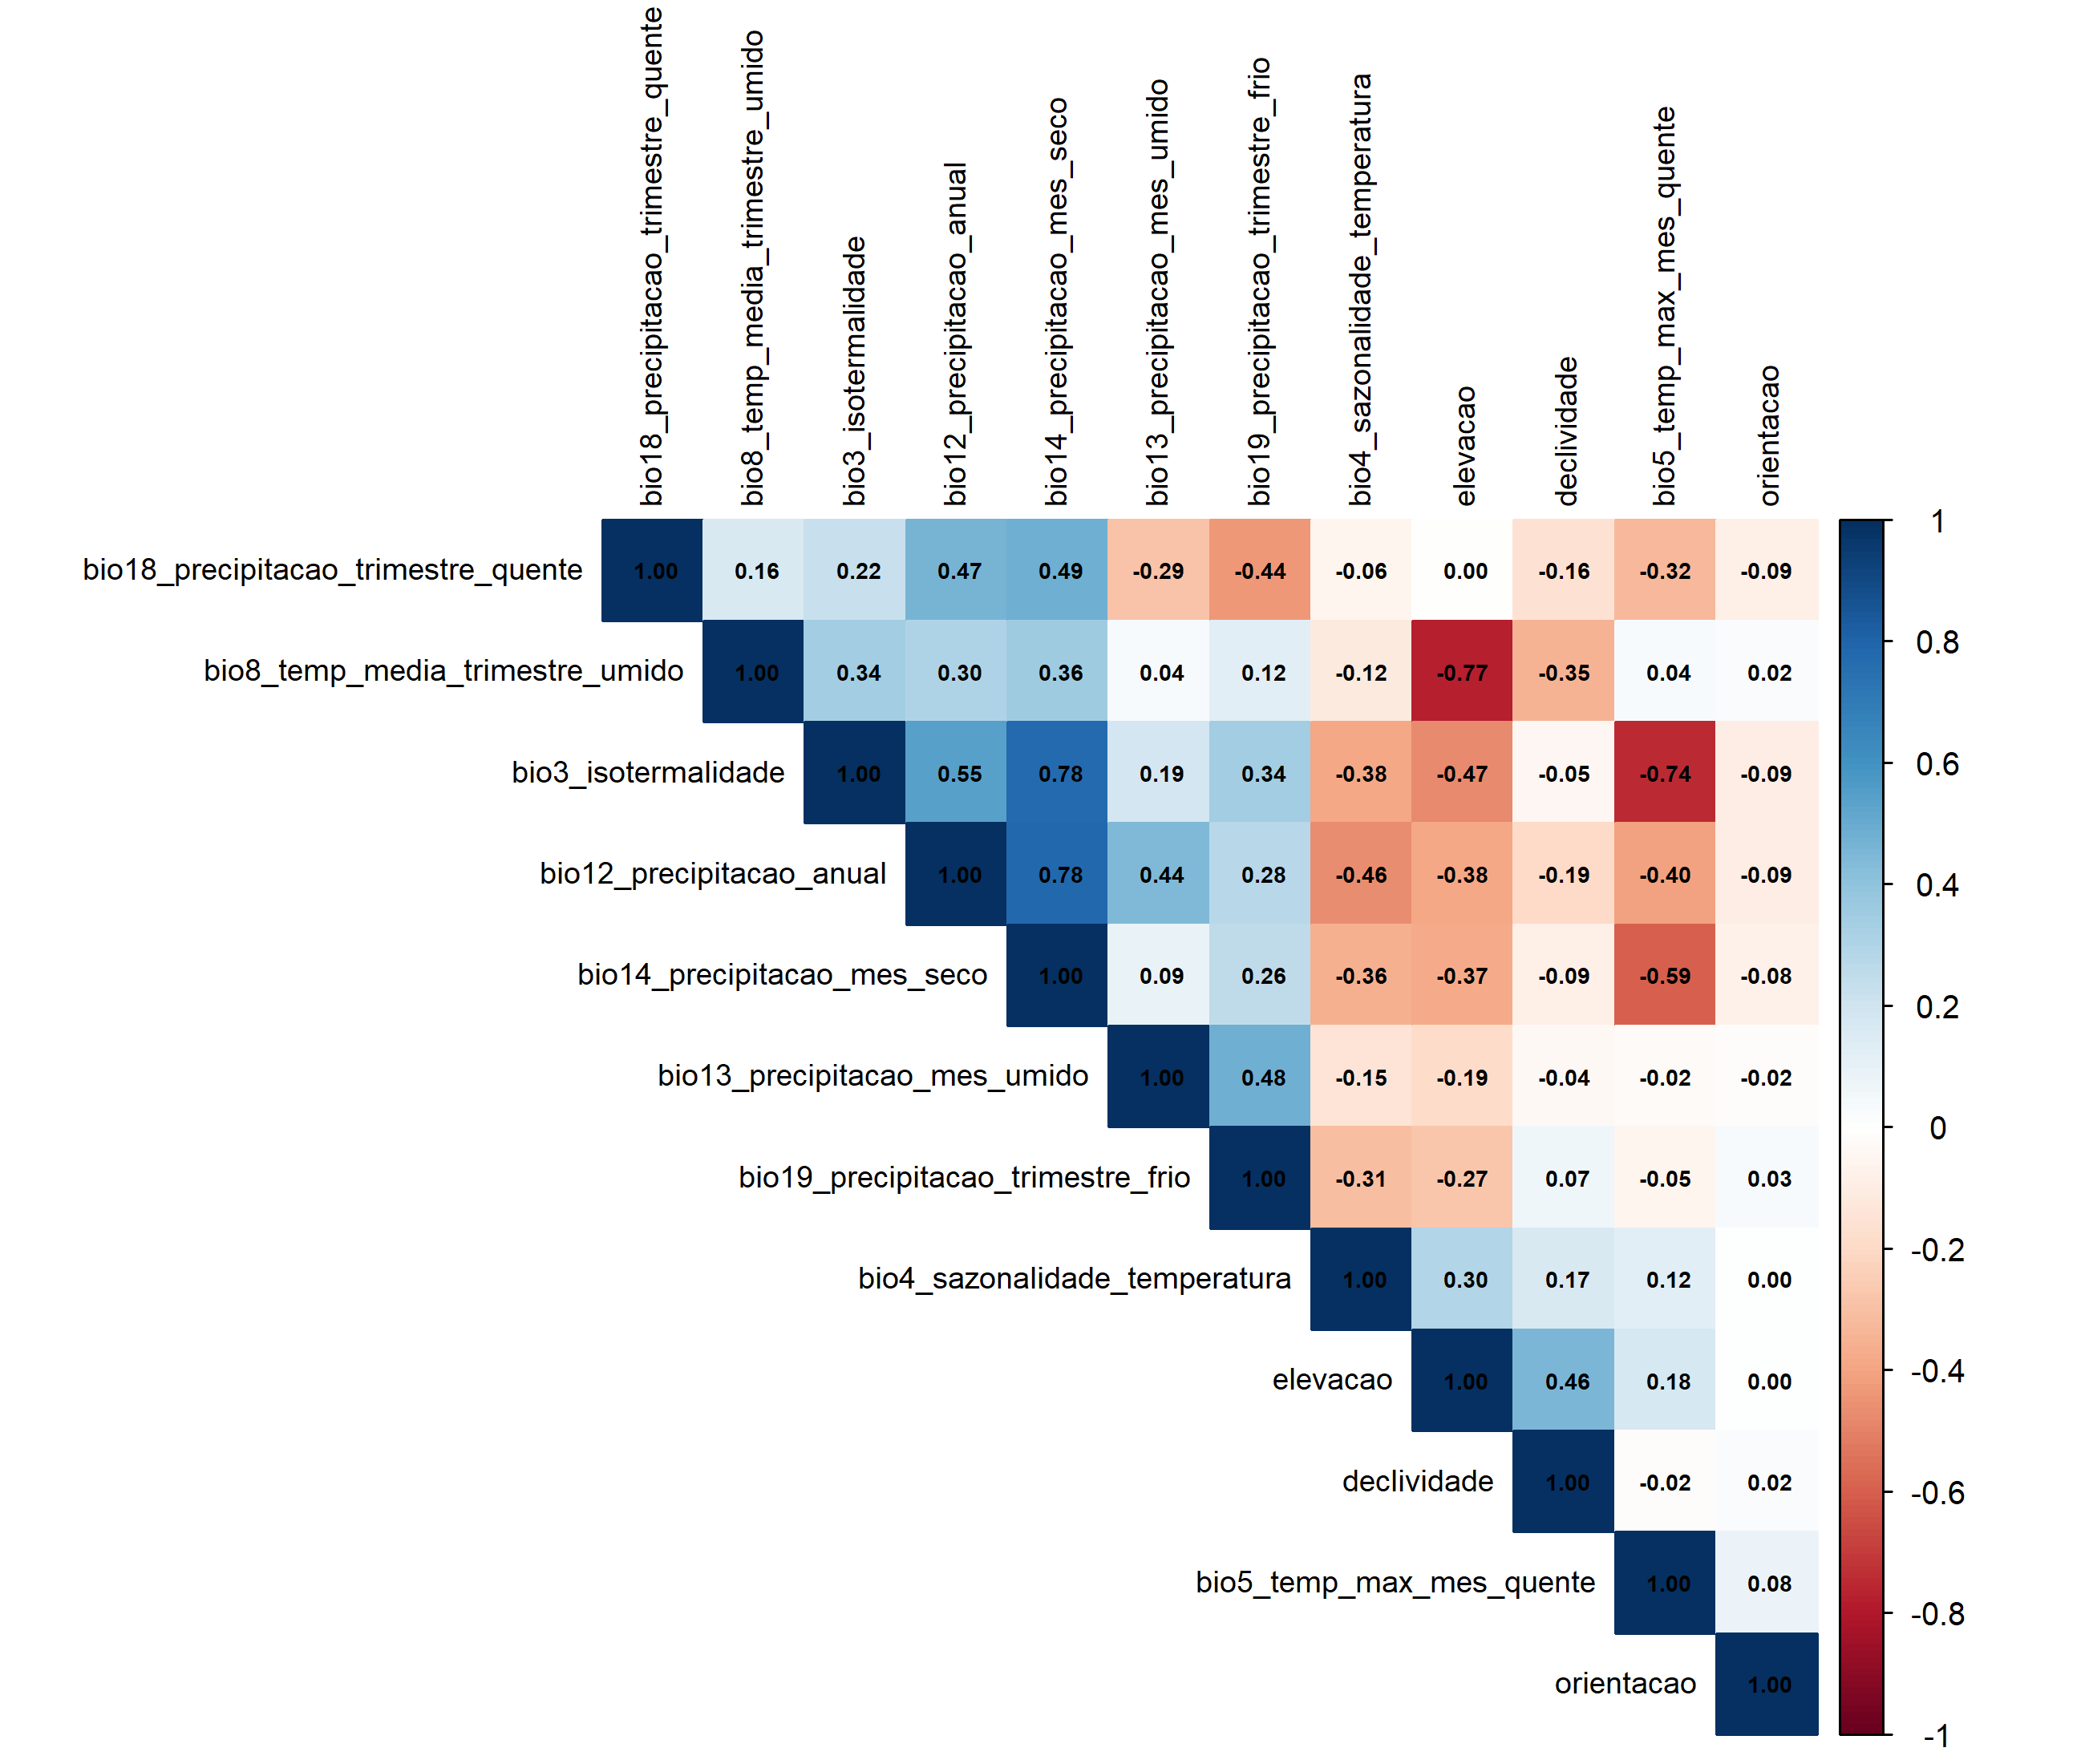
\includegraphics[width=0.95\textwidth]{figuras/unidade04/unidade04_corrplot_correlacao.png}
  \caption{Graphical representation of correlations among environmental variables. More intense colors denote stronger correlations, whereas values near zero indicate greater independence.}
  \label{fig:unidade04_corrplot}
\end{figure}

\begin{figure}[H]
  \centering
  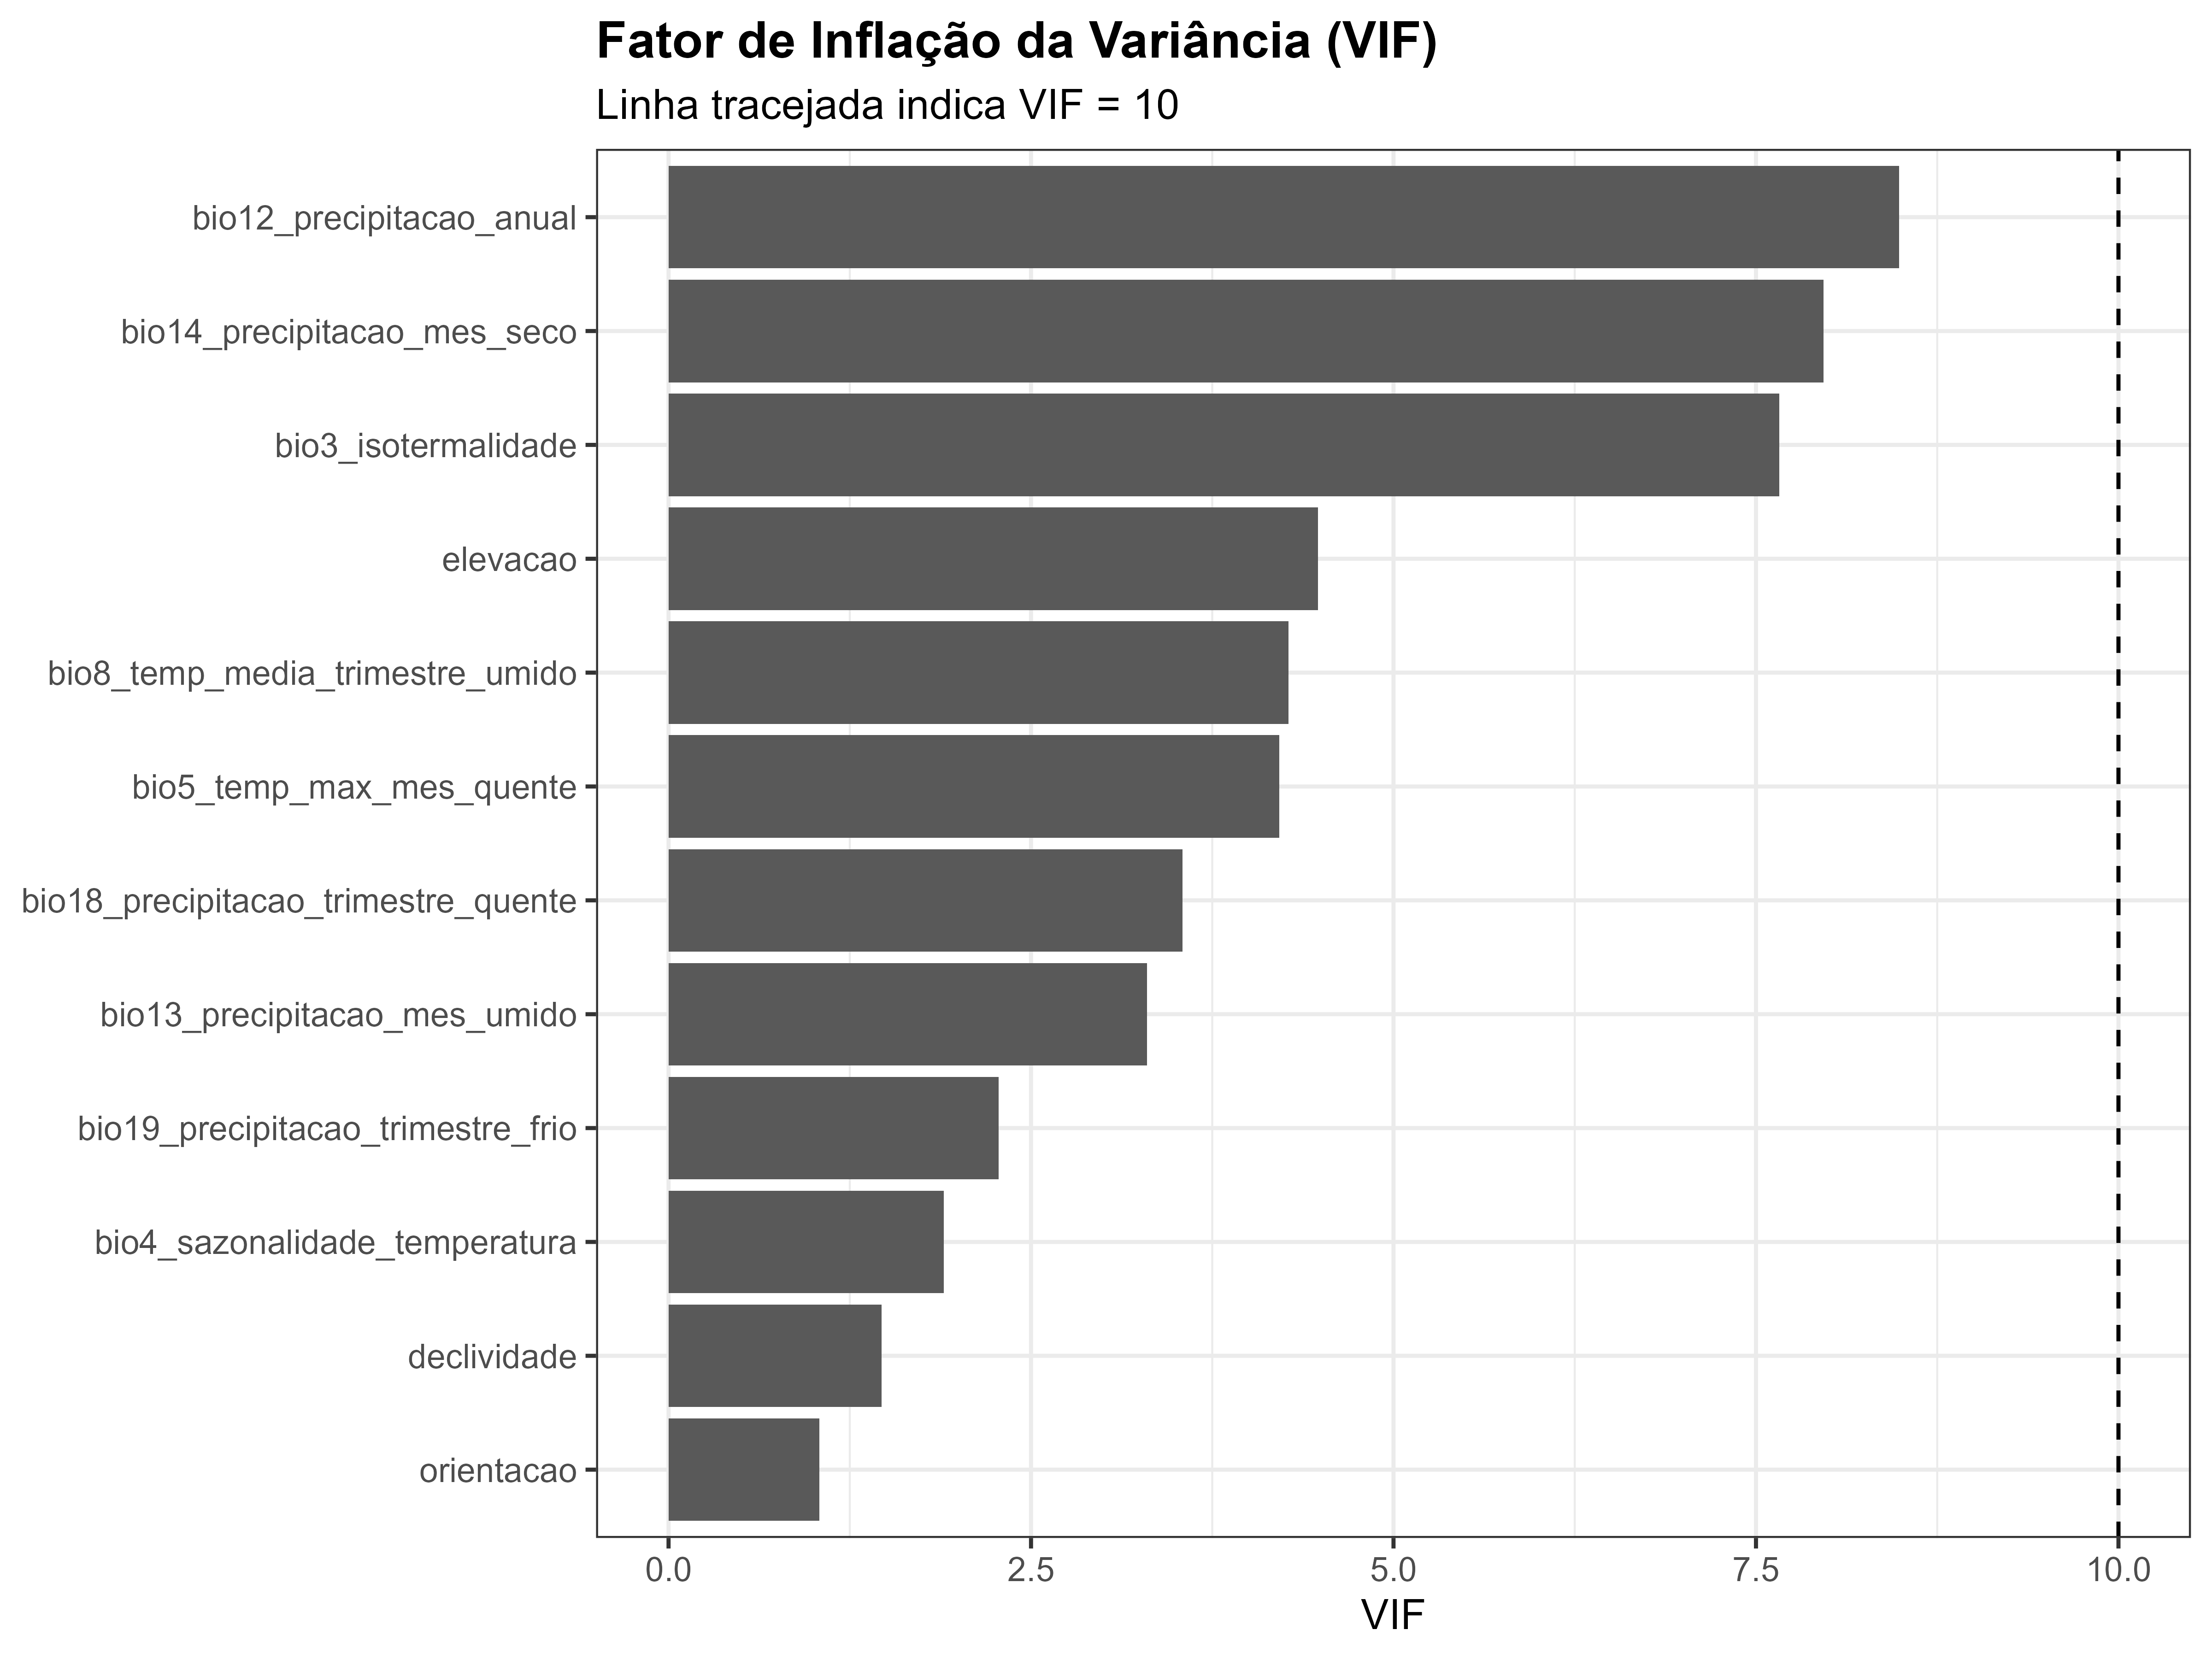
\includegraphics[width=0.85\textwidth]{figuras/unidade04/unidade04_vif_variaveis.png}
  \caption{Variance inflation factor values for the evaluated environmental variables. The dashed line is the operational threshold used to identify excessive multicollinearity.}
  \label{fig:unidade04_vif}
\end{figure}

\begin{aplicacao}
Figures~\ref{fig:unidade04_matriz_correlacao} and
\ref{fig:unidade04_corrplot} identify groups of variables carrying similar
information. Retaining strongly correlated predictors can impede ecological
interpretation and destabilize spatial and temporal projections.
\end{aplicacao}

\begin{aplicacao}
VIF quantifies how much the variance associated with a predictor is inflated by
correlation with other predictors. High values indicate statistical redundancy
and suggest removing the variable or replacing it with a more ecologically
representative alternative.
\end{aplicacao}

\section{Selecting Environmental Variables}

Variable selection must balance ecological relevance, data quality, and
statistical redundancy. Automatic removal based solely on thresholds can yield
ecologically weak models, whereas retaining redundant variables makes models
difficult to interpret.

A useful workflow begins with a broad candidate set, provides an ecological
justification for each predictor group, and then applies correlation and VIF
filters. When variables are correlated, priority should be given to the one
more directly linked to ecological processes, more stable through time, better
resolved, or subject to less measurement error.

\begin{atencao}[title={\faExclamationTriangle\quad Do not let the algorithm alone select the predictors}]
Automated selection may discard ecologically important variables while
retaining statistically convenient but biologically fragile ones. Predictor
selection must be documented and justified.
\end{atencao}

\rscriptfile{scripts/unidade04/05_selecao_variaveis.R}

\begin{figure}[H]
  \centering
  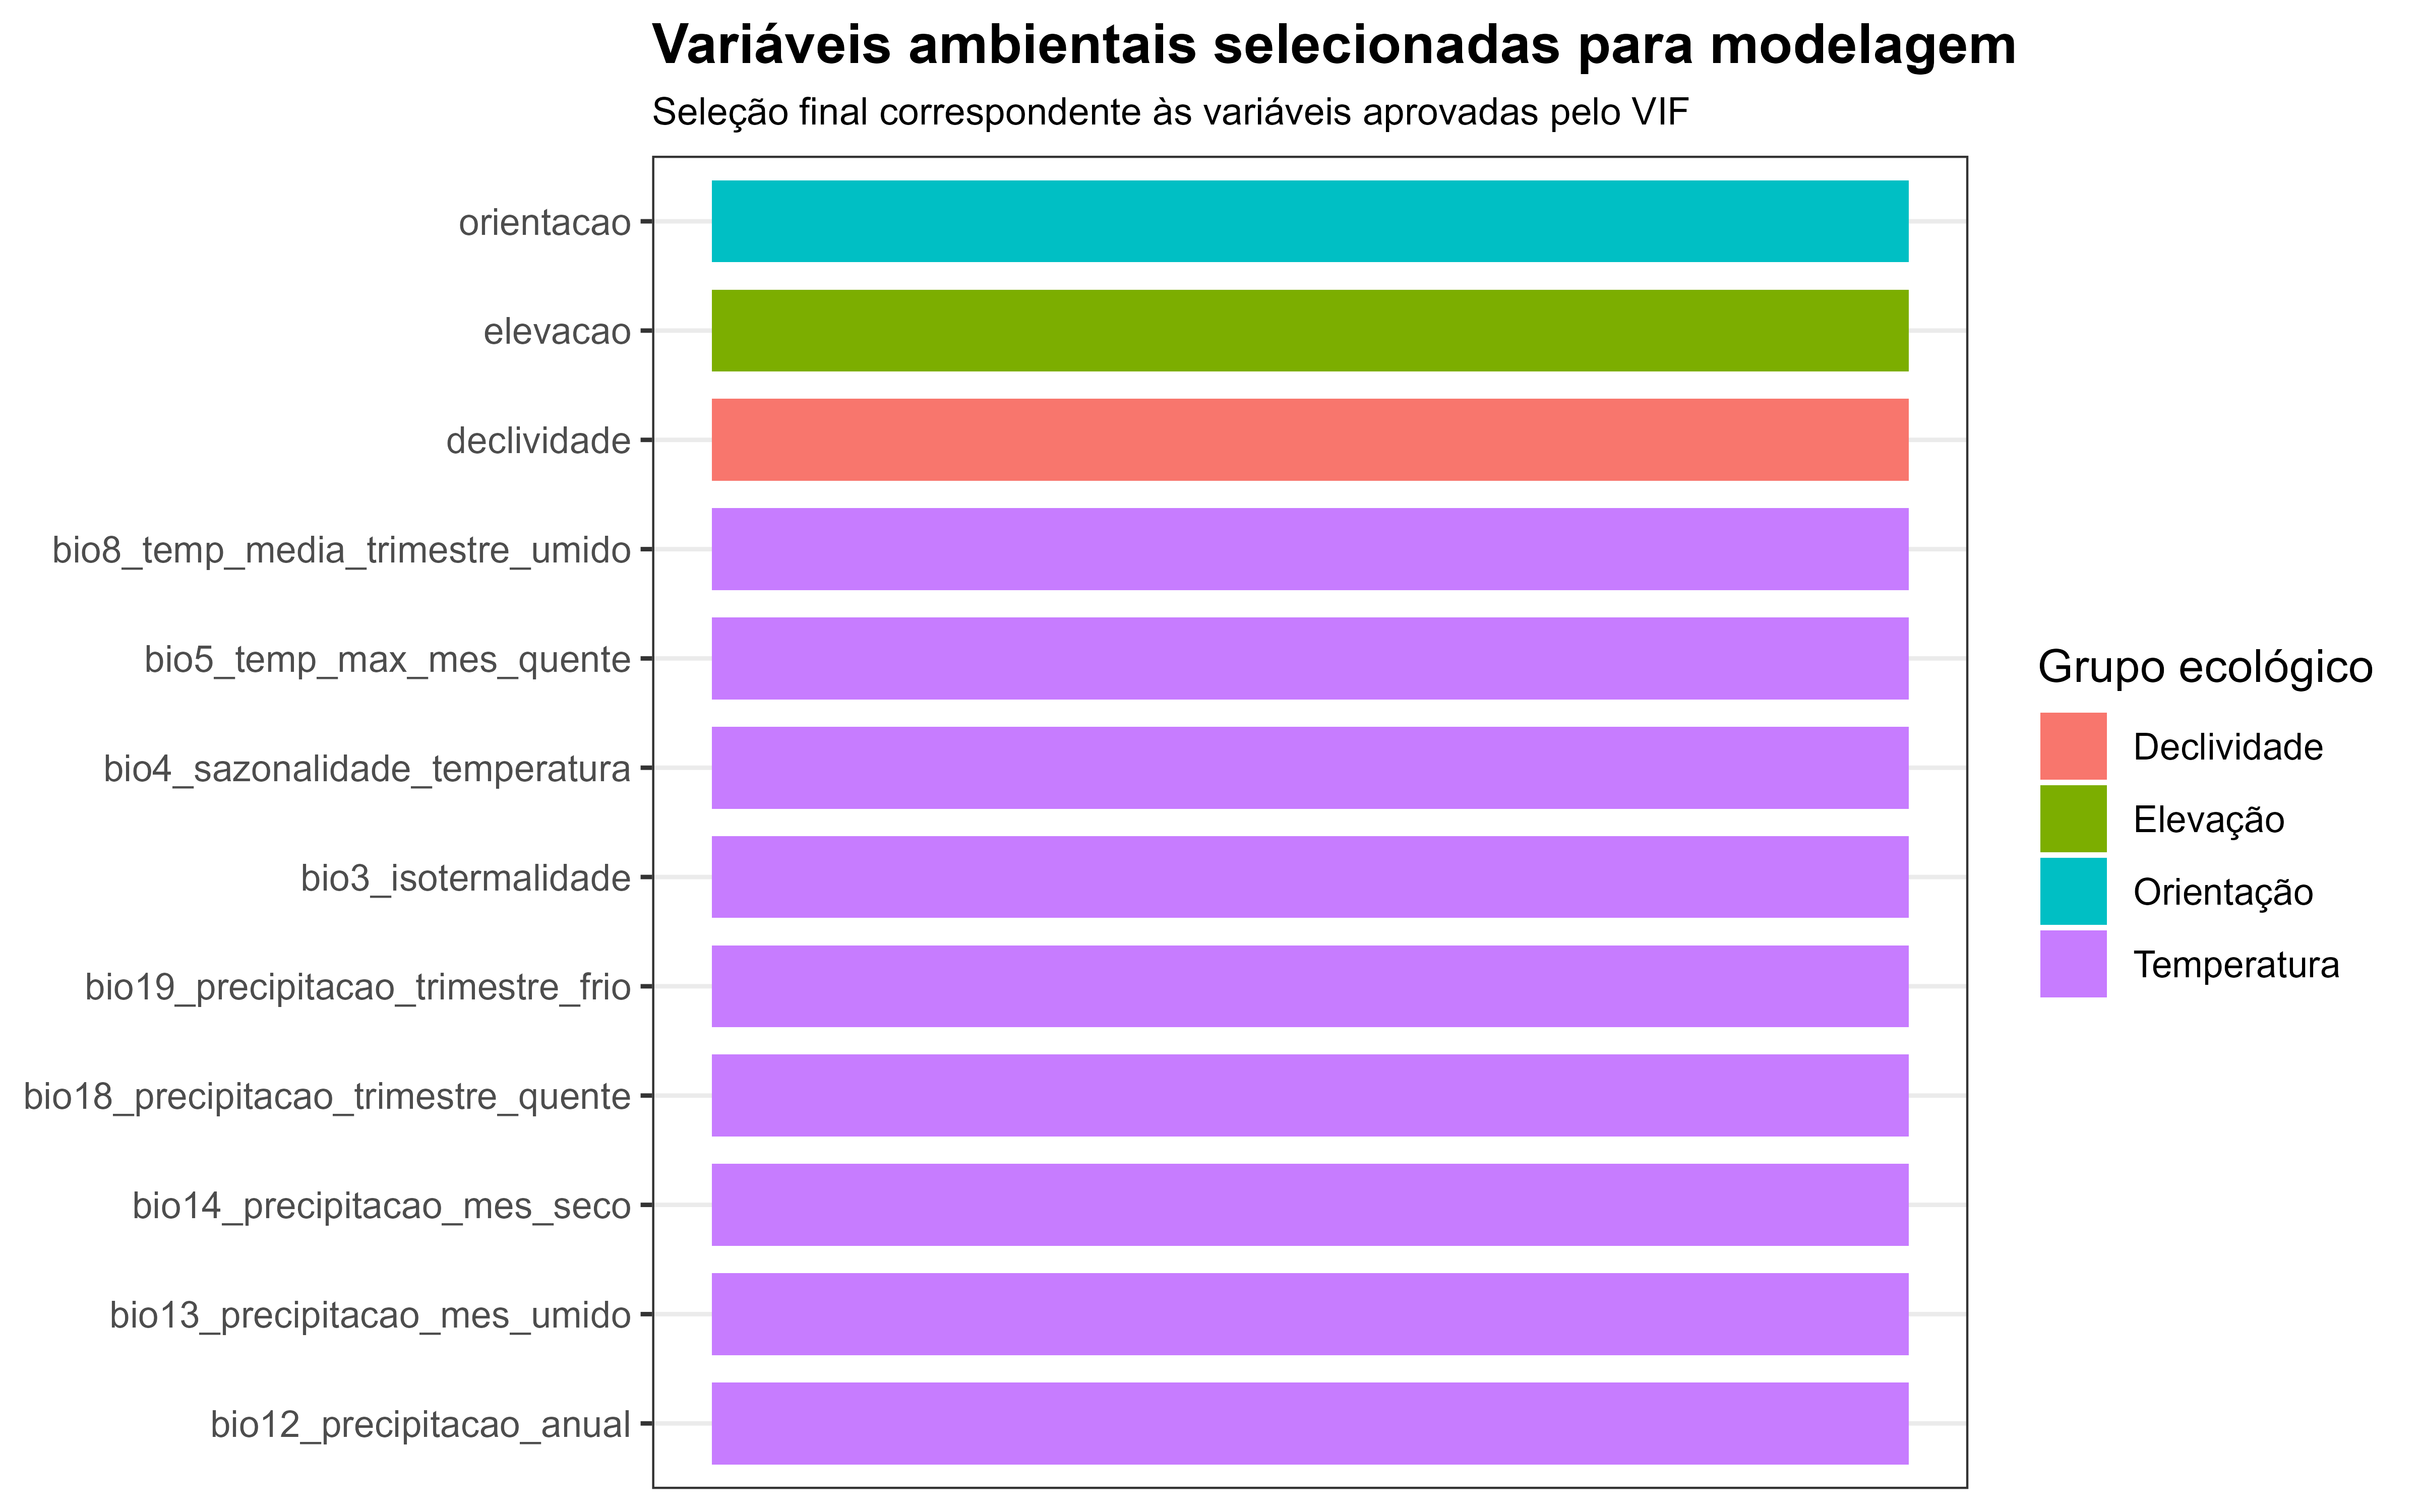
\includegraphics[width=0.85\textwidth]{figuras/unidade04/unidade04_variaveis_selecionadas.png}
  \caption{Final environmental predictors selected after correlation analysis, VIF diagnosis, and ecological interpretation. These variables are used to fit species distribution models in subsequent chapters.}
  \label{fig:unidade04_variaveis_final}
\end{figure}

\section{PCA in Species Distribution Modeling}

Principal component analysis is a dimensionality-reduction method that
transforms correlated variables into orthogonal axes. These principal
components are uncorrelated linear combinations of the original variables.

PCA can provide a compact representation of environmental space when
collinearity is strong. Its disadvantage is reduced direct ecological
interpretability: a component represents a combination of variables rather than
a simple gradient such as temperature or precipitation.

\begin{conceito}[title={\faBook\quad PCA as orthogonalization}]
PCA does not select variables. It transforms correlated variables into
independent axes. This reduces collinearity but requires care when interpreting
the resulting components ecologically.
\end{conceito}

\rscriptfile{scripts/unidade04/06_pca_variaveis.R}

\begin{figure}[H]
  \centering
  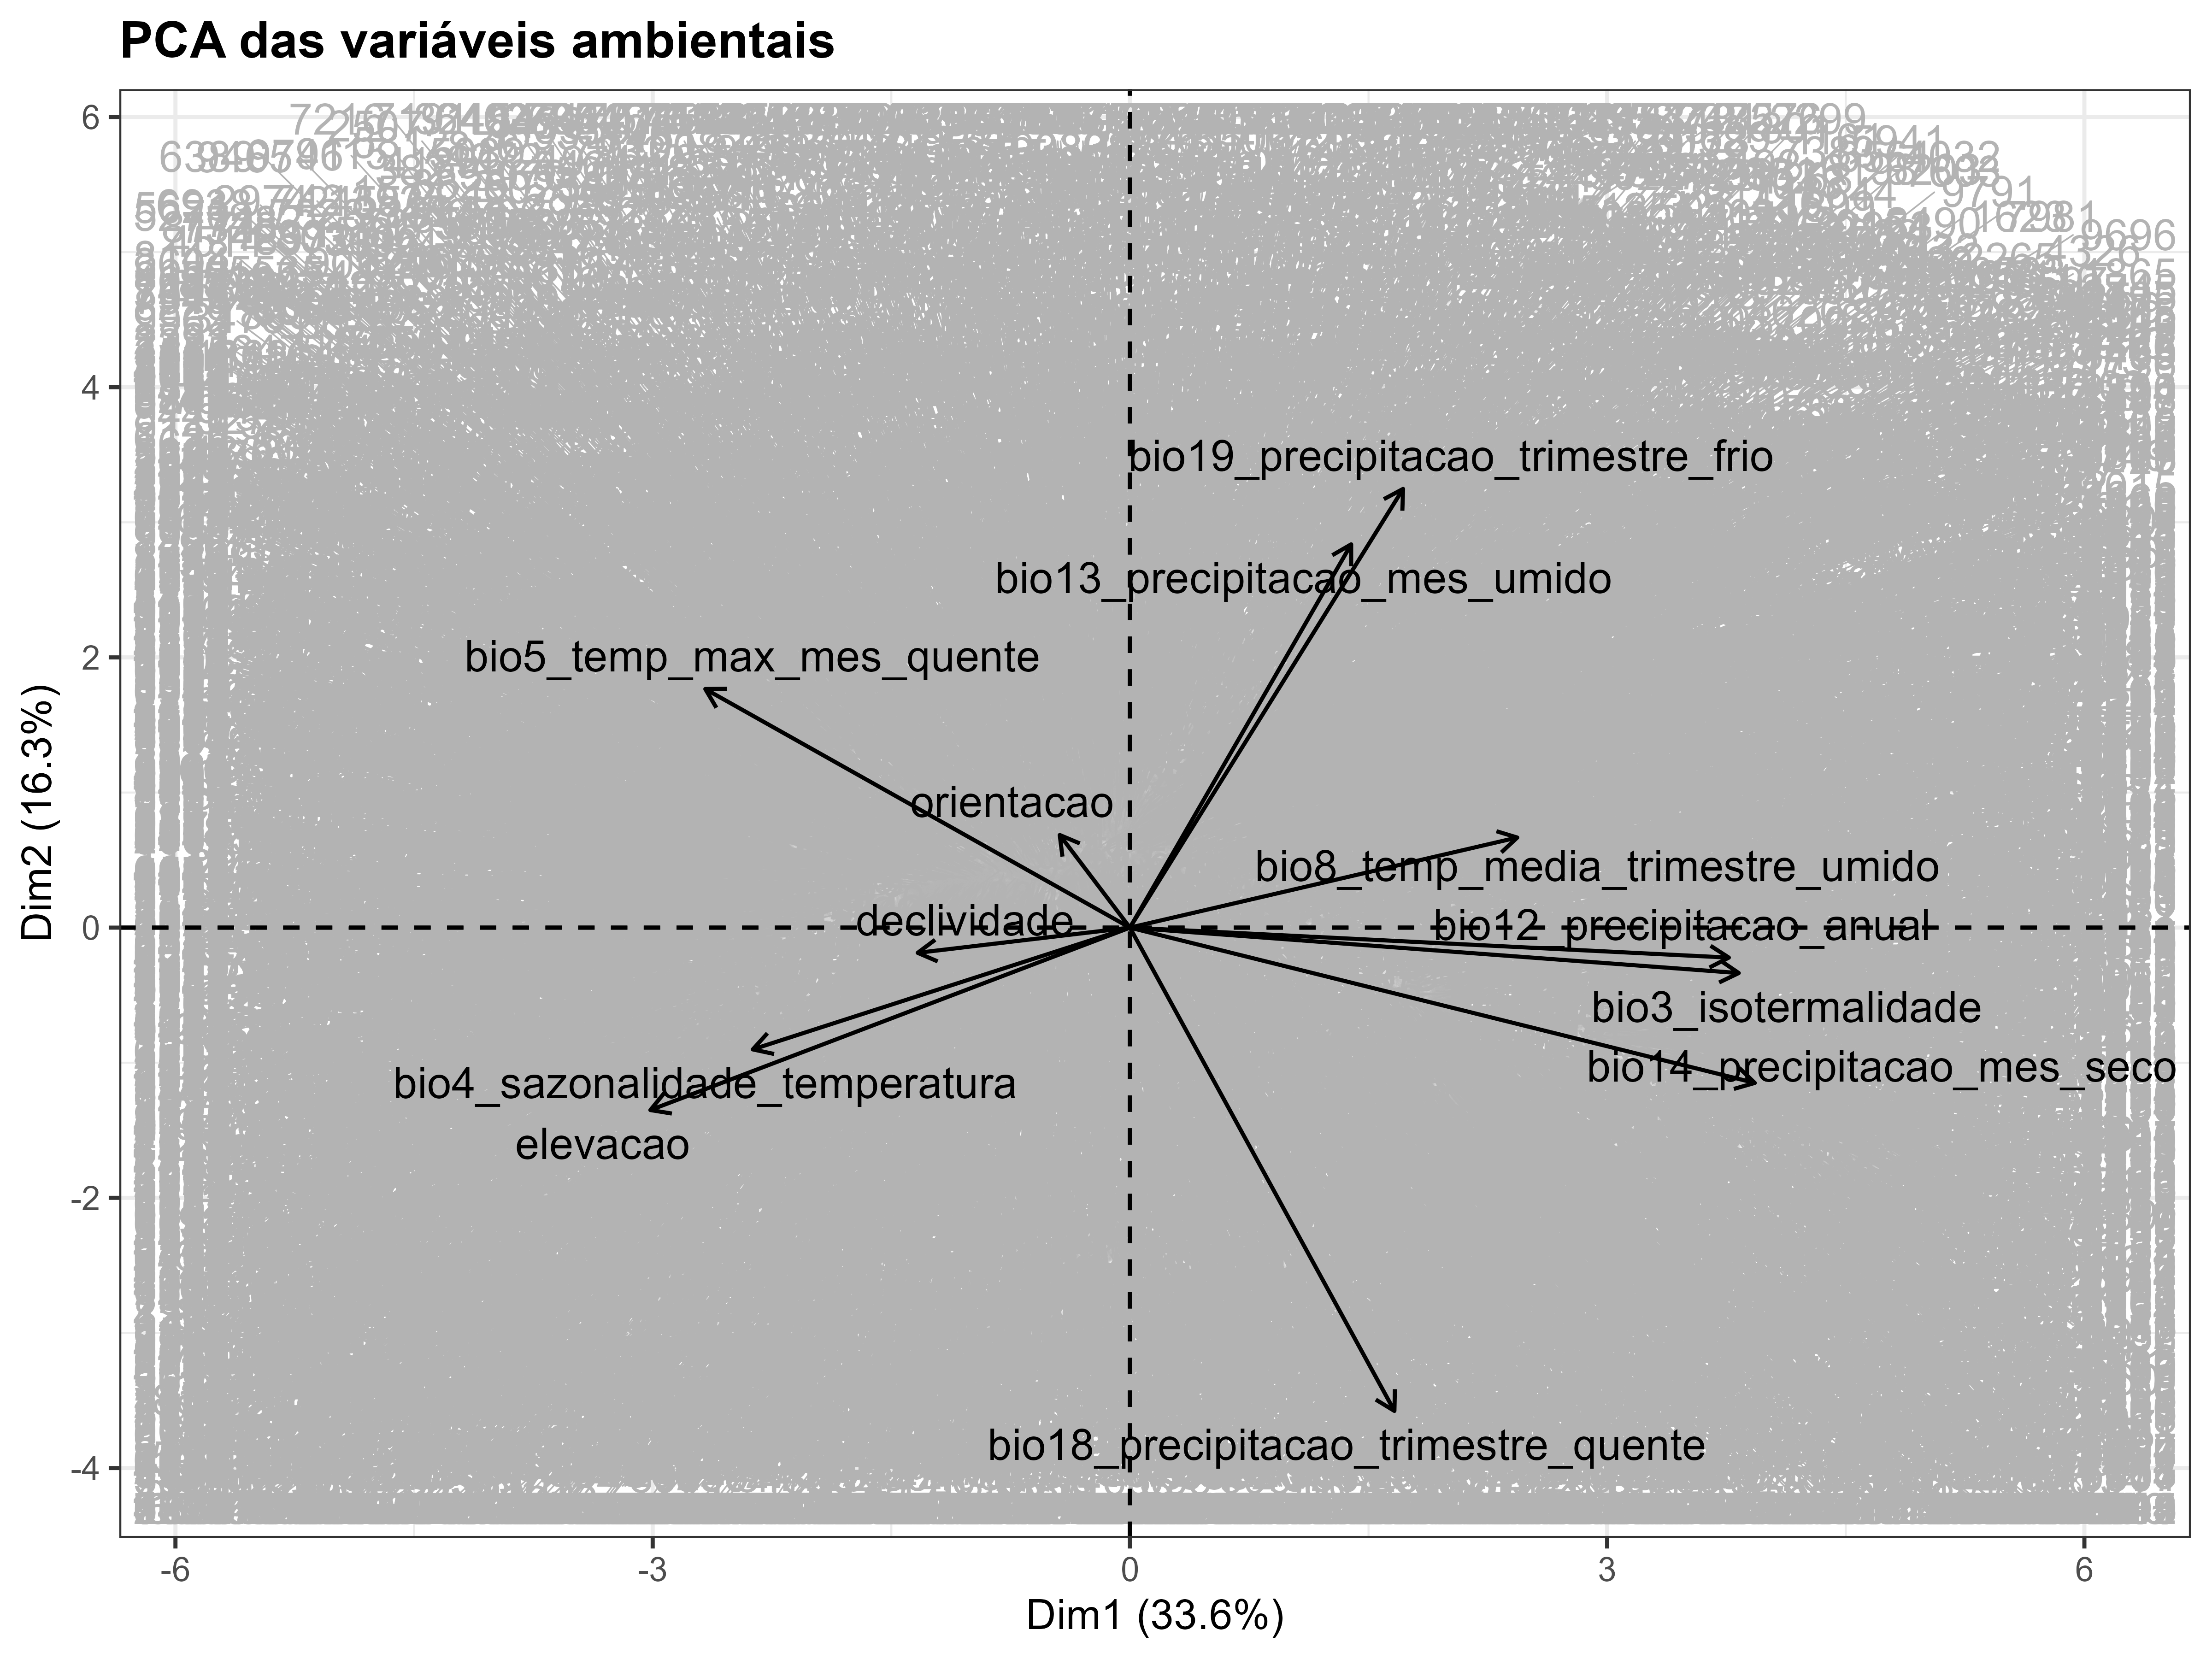
\includegraphics[width=0.90\textwidth]{figuras/unidade04/unidade04_pca_biplot_variaveis.png}
  \caption{Principal component analysis of environmental variables used in the case study. Vectors show the contribution of each variable to the principal environmental gradients of the Amazon biome.}
  \label{fig:unidade04_pca_biplot}
\end{figure}

\begin{figure}[H]
  \centering
  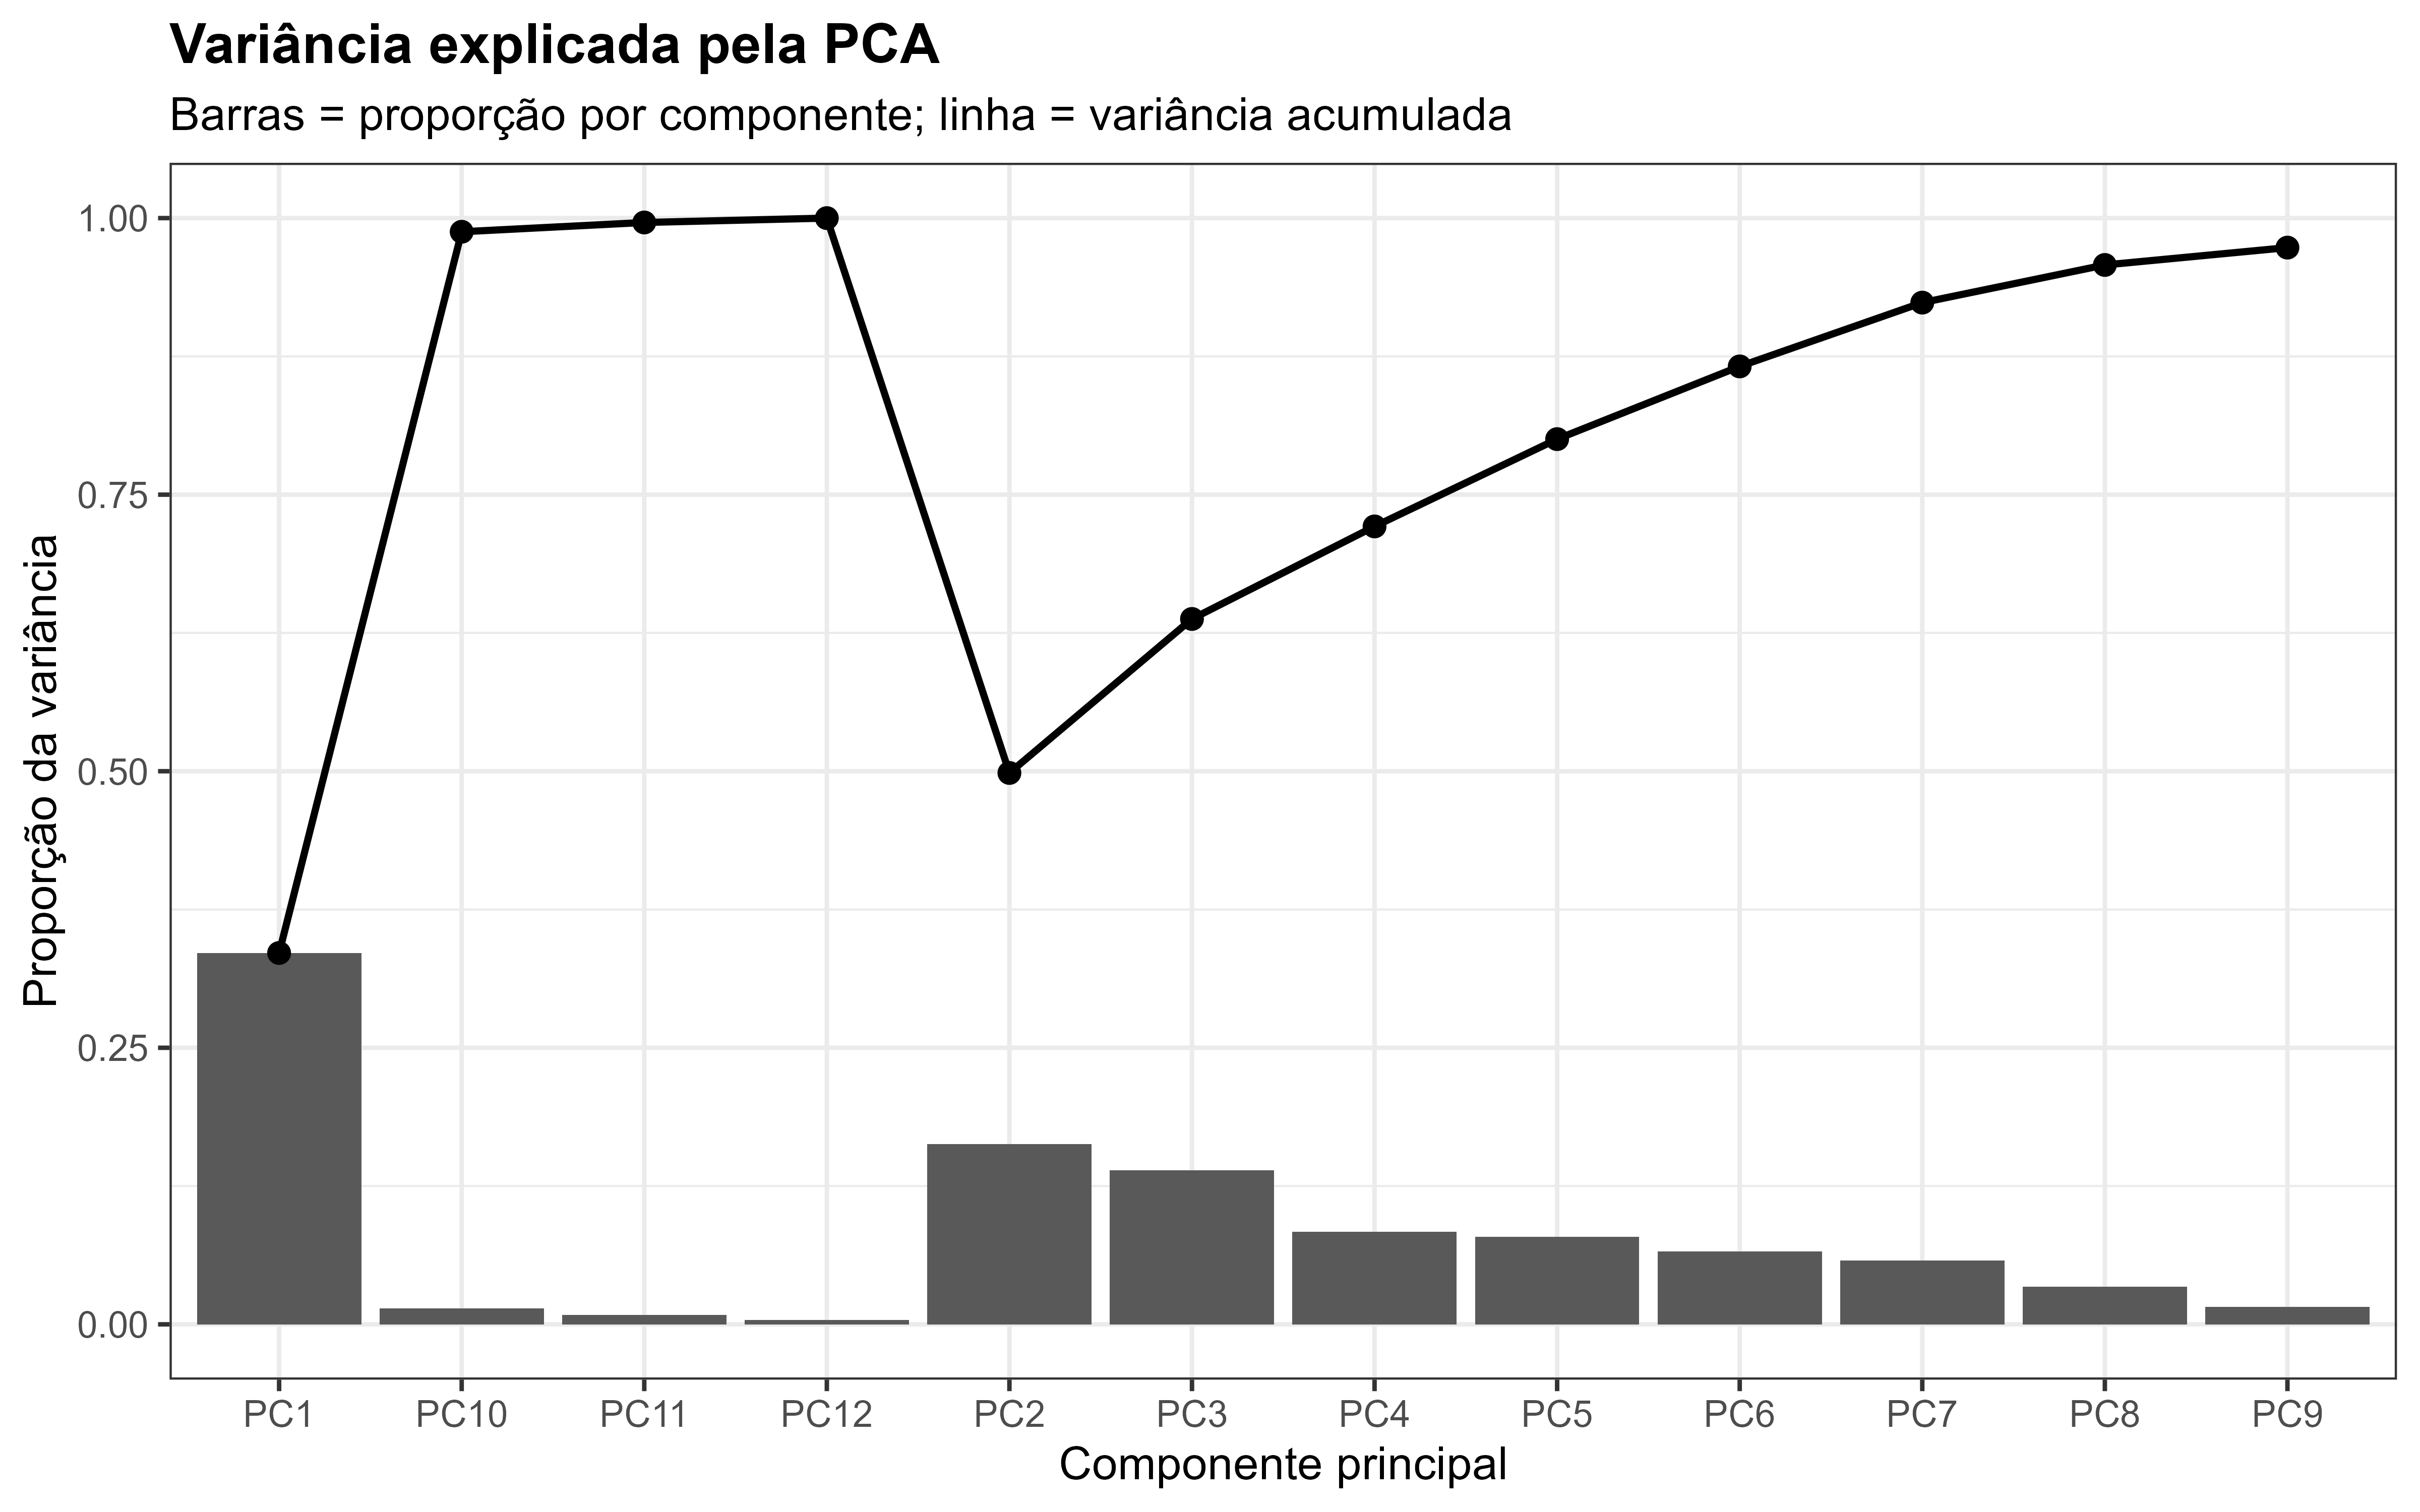
\includegraphics[width=0.80\textwidth]{figuras/unidade04/unidade04_pca_variancia.png}
  \caption{Proportion of variance explained by the principal components. Bars show the contribution of each axis and the line shows cumulative explained variance.}
  \label{fig:unidade04_pca_variancia}
\end{figure}

\begin{aplicacao}
Figures~\ref{fig:unidade04_pca_biplot} and
\ref{fig:unidade04_pca_variancia} show that a small number of principal axes can
represent much of Amazonia's environmental structure. PCA does not replace
ecological variable selection, but helps diagnose redundancy and interpret the
gradients structuring the distribution of \textit{Dinizia excelsa}.
\end{aplicacao}

\section{Integrated Pipeline}

The final script combines all Chapter 4 steps: preparation of the environmental
variables, correlation analysis, VIF diagnosis, variable selection, and PCA.

\rscriptfile{scripts/unidade04/08_pipeline_multicolinearidade.R}

\section{Chapter Summary}

Multicollinearity is central to SDM because it affects interpretation,
stability, and transferability. Correlation, VIF, and PCA are complementary.
Correlation diagnoses pairwise redundancy; VIF assesses multivariate
redundancy; and PCA transforms correlated variables into independent axes.
Whether variables should be removed or transformed depends on the scientific
question, algorithm, need for ecological interpretation, and intended spatial
or temporal projection.

\begin{conceito}[title={\faBook\quad Key message from Chapter 4}]
Variable selection is not merely a statistical procedure. Its purpose is to
construct a predictor set representing the main ecological filters associated
with species distribution, while avoiding excessive redundancy and improving
model interpretability. The variables selected here are used in Chapters 5--17
for model fitting, evaluation, climate projection, and conservation applications.
\end{conceito}

\begin{aplicacao}
From this point onward, the selected predictors constitute a refined ecological
hypothesis about the factors influencing \textit{Dinizia excelsa} in Amazonia.
The next chapter integrates these predictors with the accessible area ($M$) in
the BAM framework.
\end{aplicacao}

\section{Review Exercises}

\begin{enumerate}
  \item What is multicollinearity, and why is it common among environmental variables?
  \item Distinguish Pearson from Spearman correlation.
  \item Why should two strongly correlated variables not automatically be retained in one model?
  \item Explain the meaning of VIF.
  \item How do correlation and VIF diagnostics differ?
  \item When can PCA be useful in SDM?
  \item Discuss one ecological disadvantage of using principal components as predictors.
\end{enumerate}
